\documentclass{report}

\usepackage{fancyhdr}
\usepackage{parskip}
\usepackage{amsmath}
\usepackage[linguistics]{forest}
\usepackage[shortlabels]{enumitem}
\usepackage{caption}
\usepackage{float}
\usepackage{tikz}
\usetikzlibrary{automata, positioning, arrows}
\tikzset{
->, % makes the edges directed
>=stealth, % makes the arrow heads bold
node distance=2cm, % specifies the minimum distance between two nodes. Change if necessary.
every state/.style={thick, fill=gray!10}, % sets the properties for each ’state’ node
initial text=$ $, % sets the text that appears on the start arrow
}

\newcommand\Mydiv[2]{%
$\strut#1$\kern.25em\smash{\raise.3ex\hbox{$\big)$}}$\mkern-8mu
        \overline{\enspace\strut#2}$}

\begin{document}
    The entire idea behind NFA $\rightarrow$ Regular Expression conversion is to label edges by regular expressions instead of just single symbols.
    
    By the end of the conversion we will have just two nodes, $I$ and $F$ with one big long regexp connecting them.

    But problem 1(a) is harder. Here is a problem similar to 1(a) that I can solve without earning an academic integrity violation:

    \textbf{Find a regular expression for the complement of $\mathbf{L\left( (aa^* b) (bb^* a) \right)}$}

    The first step is to convert that regular expression to an NFA, which we will change the accepting states of to make it accept the inverse.

    That NFA for $(aa^* b) (bb^* a)$ looks like:

    \begin{figure}[H] % ’ht’ tells LaTeX to place the figure ’here’ or at the top of the page
        \centering % centers the figure
        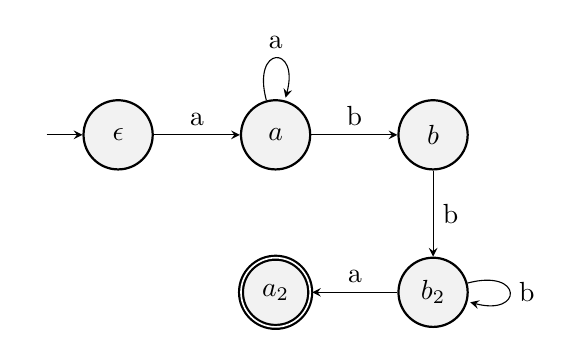
\begin{tikzpicture}

            \node[state, initial] (e) {$\epsilon$};

            \node [state, right of=e] (a) {$a$};
            \node [state, right of=a] (b) {$b$};
            \node [state, right of=a, yshift=-2cm] (b2) {$b_2$};
            \node [state, left of=b2, accepting] (a2) {$a_2$};

            \draw   (e) edge[above] node{a} (a)
                    (a) edge[above] node{b} (b)
                    (a) edge[loop above] node{a} (a)
                    (b) edge[right] node{b} (b2)
                    (b2) edge[loop right] node{b} (b2)
                    (b2) edge[above] node{a} (a2)
                    ;
        \end{tikzpicture}
        \caption*{}
        \label{fig:basicnfa}
    \end{figure}

    If we want the NFA for its complement, we just change which states are accepting (the accepting states are double-ringed. We notate it in class with a line away but I don't know how to do that in latex):


    \begin{figure}[H] % ’ht’ tells LaTeX to place the figure ’here’ or at the top of the page
        \centering % centers the figure
        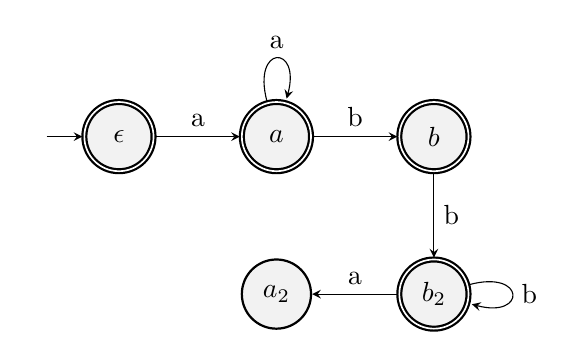
\begin{tikzpicture}

            \node[state, initial, accepting] (e) {$\epsilon$};
            \node [state, right of=e, accepting] (a) {$a$};
            \node [state, right of=a, accepting] (b) {$b$};
            \node [state, right of=a, yshift=-2cm, accepting] (b2) {$b_2$};
            \node [state, left of=b2] (a2) {$a_2$};

            \draw   (e) edge[above] node{a} (a)
                    (a) edge[above] node{b} (b)
                    (a) edge[loop above] node{a} (a)
                    (b) edge[right] node{b} (b2)
                    (b2) edge[loop right] node{b} (b2)
                    (b2) edge[above] node{a} (a2)
                    ;
        \end{tikzpicture}
        \caption*{}
        \label{fig:basicnfacomp}
    \end{figure}

    Now this accepts the complement of $(aa^* b) (bb^* a)$. It will accept anything so long as it doesn't reach $a_2$.

    Now let's run the NFA $\rightarrow$ regex conversion. I'll save us both some time and just show the answer, which I'll get by removing nodes and re-labeling edges accordingly:
    % \begin{figure}[H] % ’ht’ tells LaTeX to place the figure ’here’ or at the top of the page
    %     \centering % centers the figure
    %     \begin{tikzpicture}

    %         \node[state, initial] (i) {$I$};
    %         \node[state, accepting, right of=i] (e) {$\epsilon$};
    %         \node [state, right of=e, accepting] (a) {$a$};
    %         \node [state, right of=a, accepting] (b) {$b$};
    %         \node [state, right of=a, yshift=-2cm, accepting] (b2) {$b_2$};
    %         \node [state, left of=b2] (a2) {$a_2$};
    %         \node[state, accepting, left of=a2] (f) {$F$};

    %         \draw   (e) edge[above] node{a} (a)
    %                 (i) edge[above] node{$\epsilon$} (e)
    %                 (a) edge[above] node{b} (b)
    %                 (a) edge[loop above] node{a} (a)
    %                 (b) edge[right] node{b} (b2)
    %                 (b2) edge[loop right] node{b} (b2)
    %                 (b2) edge[above] node{a} (a2)
    %                 (e) edge[left] node{$\epsilon$} (f)
    %                 (a) edge[above] node{$\epsilon$} (f)
    %                 (b) edge[above] node{$\epsilon$} (f)
    %                 (b2) edge[below, bend left] node{$\epsilon$} (f)
    %                 ;
    %     \end{tikzpicture}
    %     \caption*{Step 1: add $I$ and $F$ states. We have a whole bunch of states that are accepting, but they ALL still need epsilon transitions to $F$}
    %     \label{fig:s1}
    % \end{figure}

    % \begin{figure}[H] % ’ht’ tells LaTeX to place the figure ’here’ or at the top of the page
    %     \centering % centers the figure
    %     \begin{tikzpicture}

    %         \node[state, initial] (i) {$I$};
    %         \node [state, right of=e, accepting] (a) {$a$};
    %         \node [state, right of=a, accepting] (b) {$b$};
    %         \node [state, right of=a, yshift=-2cm, accepting] (b2) {$b_2$};
    %         \node [state, left of=b2] (a2) {$a_2$};
    %         \node[state, accepting, left of=a2] (f) {$F$};

    %         \draw   
    %                 (i) edge[above] node{$a$} (a)
    %                 (a) edge[above] node{b} (b)
    %                 (a) edge[loop above] node{a} (a)
    %                 (b) edge[right] node{b} (b2)
    %                 (b2) edge[loop right] node{b} (b2)
    %                 (b2) edge[above] node{a} (a2)
    %                 (i) edge[above] node{$\epsilon$} (f)
    %                 (a) edge[above] node{$\epsilon$} (f)
    %                 (b) edge[above] node{$\epsilon$} (f)
    %                 (b2) edge[below, bend left] node{$\epsilon$} (f)
    %                 ;
    %     \end{tikzpicture}
    %     \caption*{Step 2: remove nodes one by one, let's start with the $\epsilon$ node. $I$ is the only node that goes into $\epsilon$, and the $\epsilon$ node outputs to $a$ and $F$, so we need to add the correct path from $I$ to those nodes}
    %     \label{fig:s1}
    % \end{figure}

    % \begin{figure}[H] % ’ht’ tells LaTeX to place the figure ’here’ or at the top of the page
    %     \centering % centers the figure
    %     \begin{tikzpicture}

    %         \node[state, initial] (i) {$I$};
    %         \node [state, right of=a, accepting] (b) {$b$};
    %         \node [state, right of=a, yshift=-2cm, accepting] (b2) {$b_2$};
    %         \node [state, left of=b2] (a2) {$a_2$};
    %         \node[state, accepting, left of=a2] (f) {$F$};

    %         \draw   
    %                 (i) edge[above] node{$aa^*b$} (b)
    %                 (b) edge[right] node{b} (b2)
    %                 (b2) edge[loop right] node{b} (b2)
    %                 (b2) edge[above] node{a} (a2)
    %                 (i) edge[above] node{$\epsilon$} (f)
    %                 (i) edge[right, bend left] node[xshift=0.2cm]{$aa^*$} (f)
    %                 (b) edge[above] node{$\epsilon$} (f)
    %                 (b2) edge[below, bend left] node{$\epsilon$} (f)
    %                 ;
    %     \end{tikzpicture}
    %     \caption*{
    %         Next, let's remove the $a$ node, why not. 
    %         A goes to $b$ and $F$, so let's add edges to $I$ to simulate that, 
    %         pretending that we started at I, walked through $a$ and ended up at those two nodes.\\
    %         If we walked $I \rightarrow a \rightarrow b$, then we would have had $aa^*b$, so let's add that edge,
    %         and if we walked $I \rightarrow a \rightarrow F$, then we would only have $aa^*$, so let's add that $I$ to $F$ edge too}
    %     \label{fig:s2}
    % \end{figure}


    % \begin{figure}[H] % ’ht’ tells LaTeX to place the figure ’here’ or at the top of the page
    %     \centering % centers the figure
    %     \begin{tikzpicture}

    %         \node[state, initial] (i) {$I$};
    %         \node [state, right of=a, yshift=-2cm, accepting] (b2) {$b_2$};
    %         \node [state, left of=b2] (a2) {$a_2$};
    %         \node[state, accepting, left of=a2] (f) {$F$};

    %         \draw   
    %                 (i) edge[above, bend left] node[xshift=0.75cm]{$aa^*bb$} (b2)
    %                 (i) edge[left, bend right] node{$aa^*b$} (f)
    %                 (b2) edge[loop right] node{b} (b2)
    %                 (b2) edge[above] node{a} (a2)
    %                 (i) edge[above] node{$\epsilon$} (f)
    %                 (i) edge[right, bend left] node[xshift=0.2cm]{$aa^*$} (f)
    %                 (b2) edge[below, bend left] node{$\epsilon$} (f)
    %                 ;
    %     \end{tikzpicture}
    %     \caption*{
    %         Next on the chopping block is $b$, which goes to $b_2$ and $f$.
    %         }
    %     \label{fig:s3}
    % \end{figure}

    \begin{figure}[H] % ’ht’ tells LaTeX to place the figure ’here’ or at the top of the page
        \centering % centers the figure
        \begin{tikzpicture}

            \node[state, initial] (i) {$I$};
            \node [state, left of=b2] (a2) {$a_2$};
            \node[state, accepting, right of=i, xshift=4cm] (f) {$F$};

            \draw   
                    (i) edge[left, bend right] node{$aa^*bbb^*a$} (a2)
                    (i) edge[above] node{$\epsilon + aa^* + aa^*b + aa^*bb$} (f)
                    ;
        \end{tikzpicture}
        \caption*{}
        \label{fig:s3}
    \end{figure}

    It seems like our answer is:
    $aa^*bb + aa^*b + aa^* + \epsilon$

    But that doesn't look like the complement of $(aa^* b) (bb^* a)$ at all!
    We're looking for string that this regex doesn't match, and yet our answer
    doesn't even let us start a string with $b$, which would be an easy way to make
    a string that isn't matched by $(aa^* b) (bb^* a)$

    That's a terrible, terrible problem. We followed the algorithm! How did we get here?

    Let's look at the NFA we started the conversion with:

    \begin{figure}[H] % ’ht’ tells LaTeX to place the figure ’here’ or at the top of the page
        \centering % centers the figure
        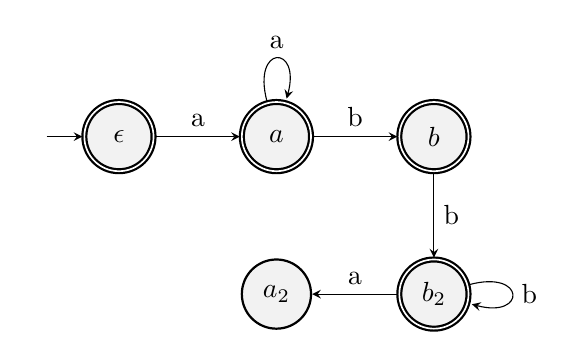
\begin{tikzpicture}

            \node[state, initial, accepting] (e) {$\epsilon$};
            \node [state, right of=e, accepting] (a) {$a$};
            \node [state, right of=a, accepting] (b) {$b$};
            \node [state, right of=a, yshift=-2cm, accepting] (b2) {$b_2$};
            \node [state, left of=b2] (a2) {$a_2$};

            \draw   (e) edge[above] node{a} (a)
                    (a) edge[above] node{b} (b)
                    (a) edge[loop above] node{a} (a)
                    (b) edge[right] node{b} (b2)
                    (b2) edge[loop right] node{b} (b2)
                    (b2) edge[above] node{a} (a2)
                    ;
        \end{tikzpicture}
        \caption*{}
        \label{fig:basicnfacomp}
    \end{figure}

    What if we plug in a string that starts with $b$?
    The machine outright rejects it, without putting it in a rejecting state.
    There's no $b$ edge away from the $\epsilon$ node, so we just stop executing.

    That's hugely, hugely bad. We took all the rejecting states from the very first machine and made them the accepting states for this machine.
    If we can reject strings without ending in a rejecting state, it's going to totally screw up our algorithm.

    That is why problem 1(a) is hard. You need to fully define the NFA that you convert your regex into.
    When we do it correctly, it looks like:

    \begin{figure}[H] % ’ht’ tells LaTeX to place the figure ’here’ or at the top of the page
        \centering % centers the figure
        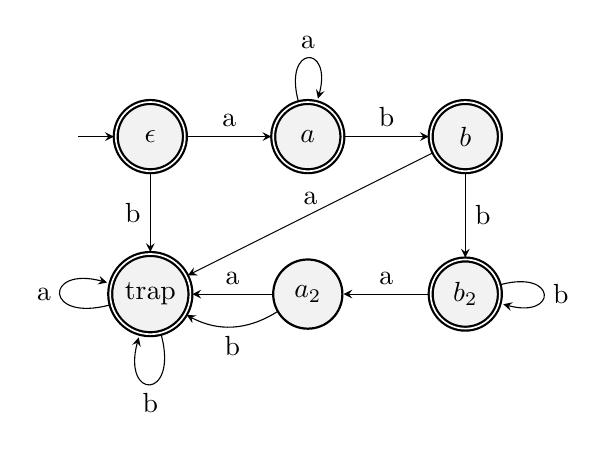
\begin{tikzpicture}

            \node[state, initial, accepting] (e) {$\epsilon$};
            \node [state, right of=e, accepting] (a) {$a$};
            \node [state, right of=a, accepting] (b) {$b$};
            \node [state, right of=a, yshift=-2cm, accepting] (b2) {$b_2$};
            \node [state, left of=b2] (a2) {$a_2$};
            \node [state, left of=a2, accepting] (trap) {trap};

            \draw   (e) edge[above] node{a} (a)
                    (a) edge[above] node{b} (b)
                    (a) edge[loop above] node{a} (a)
                    (b) edge[right] node{b} (b2)
                    (b2) edge[loop right] node{b} (b2)
                    (b2) edge[above] node{a} (a2)
                    (e) edge[left] node{b} (trap)
                    (b) edge[above] node{a} (trap)
                    (a2) edge[above] node{a} (trap)
                    (a2) edge[below, bend left] node{b} (trap)
                    (trap) edge[left, loop left] node{a} (trap)
                    (trap) edge[left, loop below] node{b} (trap)
                    ;
        \end{tikzpicture}
        \caption*{}
        \label{fig:withtrap}
    \end{figure}

    This totally changes the game. \textbf{Every node needs an edge for every symbol in the alphabet}.
    If you are going to reject a string, do it by forcing it into a rejecting state (like trap here).
    This is because you complement the NFA by marking all rejecting states accepting, allowing you to accept the strings you would normally reject.
    You just cannot do that if you don't have a rejecting state to end on.

    Let's walk through the process with the correct NFA.

    \begin{figure}[H] % ’ht’ tells LaTeX to place the figure ’here’ or at the top of the page
        \centering % centers the figure
        \caption*{Add $I$ and $F$ (it's too crowded to add epsilon transitions from all the accepting states to $F$, pretend they're there)}
        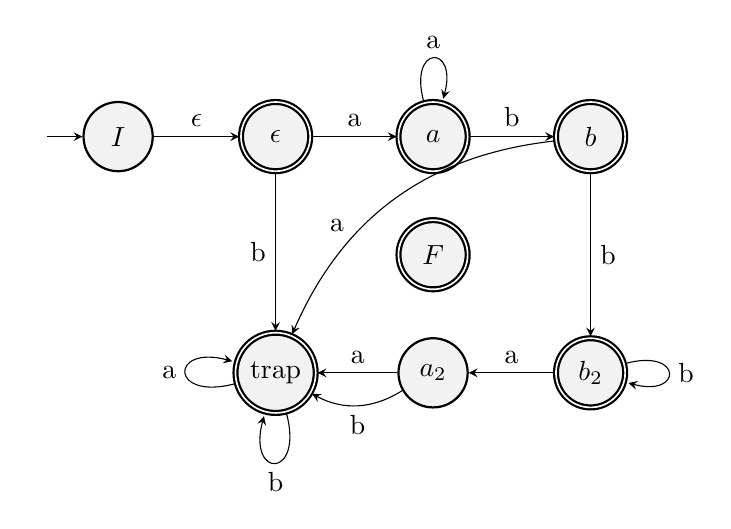
\begin{tikzpicture}

            \node[state, initial] (i) {$I$};
            \node[state, right of=i, accepting] (e) {$\epsilon$};
            \node [state, right of=e, accepting] (a) {$a$};
            \node [state, right of=a, accepting] (b) {$b$};
            \node [state, right of=a, yshift=-3cm, accepting] (b2) {$b_2$};
            \node [state, left of=b2] (a2) {$a_2$};
            \node [state, left of=a2, accepting] (trap) {trap};
            \node [state, right of=e, accepting, yshift=-1.5cm] (f) {$F$};

            \draw   (i) edge[above] node{$\epsilon$} (e)
                    (e) edge[above] node{a} (a)
                    (a) edge[above] node{b} (b)
                    (a) edge[loop above] node{a} (a)
                    (b) edge[right] node{b} (b2)
                    (b2) edge[loop right] node{b} (b2)
                    (b2) edge[above] node{a} (a2)
                    (e) edge[left] node{b} (trap)
                    (b) edge[above, bend right, pos=0.75] node[yshift=0.2cm]{a} (trap)
                    (a2) edge[above] node{a} (trap)
                    (a2) edge[below, bend left] node{b} (trap)
                    (trap) edge[left, loop left] node{a} (trap)
                    (trap) edge[left, loop below] node{b} (trap)
                    ;
        \end{tikzpicture}
        \label{fig:withtrap}
    \end{figure}
    
    \begin{figure}[H] % ’ht’ tells LaTeX to place the figure ’here’ or at the top of the page
        \centering % centers the figure
        \caption*{Remove $\epsilon$}
        \begin{tikzpicture}

            \node[state, initial] (i) {$I$};
            \node [state, right of=e, accepting] (a) {$a$};
            \node [state, right of=a, accepting] (b) {$b$};
            \node [state, right of=a, yshift=-3cm, accepting] (b2) {$b_2$};
            \node [state, left of=b2] (a2) {$a_2$};
            \node [state, left of=a2, accepting] (trap) {trap};
            \node [state, right of=e, accepting, yshift=-1.5cm] (f) {$F$};

            \draw   (i) edge[above] node{$a$} (a)
                    (i) edge[left] node{b} (trap)
                    (i) edge[above, bend right, looseness=0.5] node{$\epsilon$} (f)
                    (a) edge[above] node{b} (b)
                    (a) edge[loop above] node{a} (a)
                    (b) edge[right] node{b} (b2)
                    (b2) edge[loop right] node{b} (b2)
                    (b2) edge[above] node{a} (a2)
                    (b) edge[above, bend right, pos=0.75] node[yshift=0.2cm]{a} (trap)
                    (a2) edge[above] node{a} (trap)
                    (a2) edge[below, bend left] node{b} (trap)
                    (trap) edge[left, loop left] node{a} (trap)
                    (trap) edge[left, loop below] node{b} (trap)
                    ;
        \end{tikzpicture}
        \label{fig:withtrap}
    \end{figure}

    \begin{figure}[H] % ’ht’ tells LaTeX to place the figure ’here’ or at the top of the page
        \centering % centers the figure
        \caption*{Remove $a$, move $F$ because its getting crowded}
        \begin{tikzpicture}

            \node[state, initial] (i) {$I$};
            \node [state, right of=a, accepting] (b) {$b$};
            \node [state, right of=a, yshift=-3cm, accepting] (b2) {$b_2$};
            \node [state, left of=b2] (a2) {$a_2$};
            \node [state, left of=a2, accepting] (trap) {trap};
            \node [state, right of=e, accepting, yshift=1.5cm] (f) {$F$};

            \draw   (i) edge[above] node{$aa^*b$} (b)
                    (i) edge[left] node{b} (trap)
                    (i) edge[above, bend right, looseness=0.5] node{$\epsilon$} (f)
                    (i) edge[above, bend left, looseness=0.5, pos=0.7] node{$aa^*$} (f)
                    (b) edge[right] node{b} (b2)
                    (b2) edge[loop right] node{b} (b2)
                    (b2) edge[above] node{a} (a2)
                    (b) edge[above, bend right, pos=0.75] node[yshift=0.2cm]{a} (trap)
                    (a2) edge[above] node{a} (trap)
                    (a2) edge[below, bend left] node{b} (trap)
                    (trap) edge[left, loop left] node{a} (trap)
                    (trap) edge[left, loop below] node{b} (trap)
                    ;
        \end{tikzpicture}
        \label{fig:withtrap}
    \end{figure}

    \begin{figure}[H] % ’ht’ tells LaTeX to place the figure ’here’ or at the top of the page
        \centering % centers the figure
        \caption*{Remove $b$, collapse the edges of $F$ down to a single, nice one because it's still too crowded }
        \begin{tikzpicture}

            \node[state, initial] (i) {$I$};
            \node [state, right of=a, yshift=-3cm, accepting] (b2) {$b_2$};
            \node [state, left of=b2] (a2) {$a_2$};
            \node [state, left of=a2, accepting] (trap) {trap};
            \node [state, right of=e, accepting, yshift=1.5cm] (f) {$F$};

            \draw   (i) edge[above, bend left, pos=0.75] node[yshift=0.4cm]{$aa^*bb$} (b2)
                    (i) edge[left] node{b} (trap)
                    (i) edge[above] node[yshift=0.75cm]{$aa^*b + aa^* + \epsilon$} (f)
                    (i) edge[left, bend right, pos=0.5] node[yshift=0.2cm, xshift=-5.95]{$aa^*ba$} (trap)
                    (b2) edge[loop right] node{b} (b2)
                    (b2) edge[above] node{a} (a2)
                    (a2) edge[above] node{a} (trap)
                    (a2) edge[below, bend left] node{b} (trap)
                    (trap) edge[left, loop left] node{a} (trap)
                    (trap) edge[left, loop below] node{b} (trap)
                    ;
        \end{tikzpicture}
        \label{fig:withtrap}
    \end{figure}

    \begin{figure}[H] % ’ht’ tells LaTeX to place the figure ’here’ or at the top of the page
        \centering % centers the figure
        \caption*{Remove $b_2$}
        \begin{tikzpicture}

            \node[state, initial] (i) {$I$};
            \node [state, left of=b2] (a2) {$a_2$};
            \node [state, left of=a2, accepting] (trap) {trap};
            \node [state, right of=e, accepting, yshift=1.5cm] (f) {$F$};

            \draw   (i) edge[above, bend left, pos=0.75] node[yshift=0.4cm, xshift=1cm]{$(aa^*b) (bb^*a)$} (a2)
                    (i) edge[left] node{b} (trap)
                    (i) edge[above] node[yshift=0.75cm, xshift=-1cm]{$(aa^*b)(bb^*) + aa^*b + aa^* + \epsilon$} (f)
                    (i) edge[left, bend right, pos=0.5] node[yshift=0.2cm, xshift=-5.95]{$aa^*ba$} (trap)
                    (a2) edge[above] node{a} (trap)
                    (a2) edge[below, bend left] node{b} (trap)
                    (trap) edge[left, loop left] node{a} (trap)
                    (trap) edge[left, loop below] node{b} (trap)
                    ;
        \end{tikzpicture}
        \label{fig:withtrap}
    \end{figure}

    \begin{figure}[H] % ’ht’ tells LaTeX to place the figure ’here’ or at the top of the page
        \centering % centers the figure
        \caption*{Now remove $a_2$}
        \begin{tikzpicture}

            \node[state, initial] (i) {$I$};
            \node [state, left of=a2, accepting] (trap) {trap};
            \node [state, right of=e, accepting, yshift=1.5cm] (f) {$F$};

            \draw   (i) edge[above, bend left, pos=0.75] node[yshift=0.4cm, xshift=1.2cm]{$(aa^*b) (bb^*a) (a+b)$} (trap)
                    (i) edge[left] node{b} (trap)
                    (i) edge[above] node[yshift=0.75cm, xshift=-1cm]{$(aa^*b)(bb^*) + aa^*b + aa^* + \epsilon$} (f)
                    (i) edge[left, bend right, pos=0.5] node[yshift=0.2cm, xshift=-5.95]{$aa^*ba$} (trap)
                    (trap) edge[left, loop left] node{a} (trap)
                    (trap) edge[left, loop below] node{b} (trap)
                    ;
        \end{tikzpicture}
        \label{fig:withtrap}
    \end{figure}
    \begin{figure}[H] % ’ht’ tells LaTeX to place the figure ’here’ or at the top of the page
        \centering % centers the figure
        \caption*{Now the big boy, remove trap. Remember that all accepting states have implied epsilon transitions to $F$, so we move the rest of this monster expression to F}
        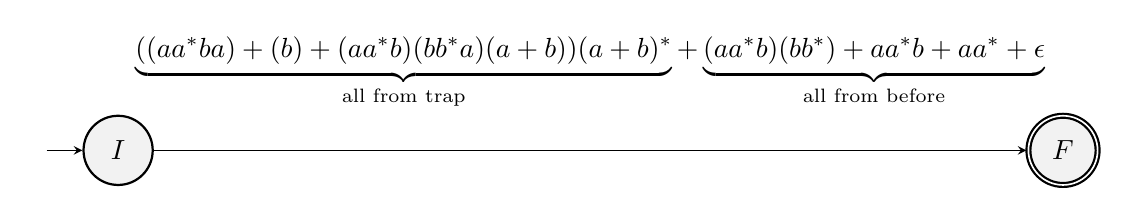
\begin{tikzpicture}

            \node[state, initial] (i) {$I$};
            \node [state, right of=i, accepting, xshift=10cm] (f) {$F$};

            \draw   (i) edge[above] node[yshift=0.4cm]{$\underbrace{((aa^*ba) + (b) + (aa^*b) (bb^*a) (a+b))(a+b)^*}_\text{all from trap} + \underbrace{(aa^*b)(bb^*) + aa^*b + aa^* + \epsilon}_\text{all from before}$} (f)
                    ;
        \end{tikzpicture}
        \label{fig:withtrap}
    \end{figure}

    And that's our regex. It's a total beast, completely gnarly, and way, way bigger and more correct than what we started with. Who knows if it's correct.
    I sure don't. I must have made a mistake somewhere, but it shows how important it is that when you convert the regex to nfa, make sure EVERY SINGLE NODE has an edge for EVERY SINGLE SYMBOL in the alphabet.
\end{document}